%===============================================================================
% (c) Dominik Harmim


\chapter{Introduction}

Bugs are an integral part of computer programs ever since the inception
of the programming discipline. Unfortunately, they are often hidden
in unexpected places, and they can lead to unexpected behaviour which
may cause significant damage. Nowadays there are many possible
ways of catching bugs in the development process. Dynamic analysis
tools or tools for automated testing are often used. These methods
are satisfactory in many cases. Nevertheless, they can still leave
too many bugs undetected, because they are able to analyse only
certain program flows, dependent on its input data. An alternative
solution is \emph{static analysis}. Of course, it has some shortages
as well. The big issue is \emph{scalability} on extensive codebases and
considerable high rate of incorrectly reported errors (so-called
\emph{false positives}, also called \emph{false alarms}).

Not long ago, Facebook introduced \emph{Facebook Infer}\,--\,a~tool for
creating \emph{highly scalable} \emph{compositional}, \emph{incremental},
and \emph{interprocedural} static analysers. Facebook Infer is a~live tool
and it is still under the development. Anyway, it is in everyday use in
Facebook itself, Spotify, Uber, Mozilla, WhatsApp and other well-known
companies. Currently, Facebook Infer provides several analysers implemented
as modules in the whole framework. These analysers check for various types
of bugs, e.g., buffer overflows, thread-safety, null-dereferencing, or
memory leaks. Facebook Infer also aims to create a~framework for building
new analysers quickly and easily. The current version of Facebook Infer still
misses better support for \emph{concurrency} bugs. While it provides a~fairly
advanced \emph{data race} analyser, it is limited to Java programs only and
fails for C~programs, which require more through manipulation with locks.

In \emph{concurrent programs}, there are often \emph{atomicity requirements}
for execution of specific sequences of instructions. Violating these
requirements may cause many kinds of problems, such as unexpected
behaviour, exceptions, segmentation faults, or other failures.
\emph{Atomicity violations} are usually not verified by compilers,
unlike syntactic or some sorts of semantic rules. Atomicity requirements,
in most cases, are not even documented. It means that typically only
programmers must take care of following these requirements. In general,
it is very difficult to avoid errors in \emph{atomicity-dependent
programs}, especially in large projects, and even harder and time-consuming
is finding and fixing these errors.

In this thesis, there is described proposal, implementation, and experimental
verification and evaluation of \emph{Atomer}\,---\,static analyser for
finding atomicity violations\,---\,which is implemented as an extension for
Facebook Infer. In particular, the concentration is put on an
\emph{atomic execution of sequences of function calls}, which is often
required, e.g., when using certain library calls. The implementation targets
to C/C++ programs that use \emph{PThread} locks.

The development of Atomer has been discussed with developers of
Facebook Infer, and it is a~part of the H2020 ECSEL project Aquas. Parts
of this paper are taken over~\cite{excel2019FBInfer}, which I~wrote
together with Vladimír Marcin and Ondřej Pavela. In~\cite{excel2019FBInfer},
there were presented preliminary results of my thesis.

The rest of the paper is organised as follows. In
Chapter~\ref{chap:prelim}, there are described all the topics
which are necessary to understand before reading the rest of the paper. In
particular, Section~\ref{sec:statAnalysisAI} deals with
\emph{static analysis} based on \emph{abstract interpretation}.
Facebook Infer, which uses abstract interpretation, is described in
Section~\ref{sec:fbinfer}. And in Section~\ref{sec:contracts}, there is
described the concept of \emph{contracts for concurrency}. A~proposal of
a~static analyser for detection of \emph{atomicity violations}, based on this
concept, is described in Chapter~\ref{chap:proposal} together with
a~description of existing analysers of a~similar kind. An implementation
of the analyser and its experimental verification and evaluation is
presented in Chapter~\ref{chap:implementExp}. Finally, Chapter~\ref{chap:conc}
concludes the paper. In addition, there are three appendices.
Appendix~\ref{chap:expRes} shows the experimental results.
Appendix~\ref{chap:memMedia} lists contents of attached memory media and
Appendix~\ref{chap:man} serves as an installation and user manual.



\chapter{Preliminaries}
\label{chap:prelim}

This chapter explains the theoretical background on which stands the
thesis. It also explains and describes the existing tools used in the
thesis. Lastly, the chapter deals with principles which this thesis
got inspired by.

The aim of this thesis is to propose a~\emph{static analyser} and implement
it in \emph{Facebook Infer}. So, in Section~\ref{sec:statAnalysisAI},
there is a~brief explanation of \emph{static analysis} itself, and then an
explanation of \emph{abstract interpretation} that is used in Facebook Infer.
Facebook Infer, its principles and features illustrate
Section~\ref{sec:fbinfer}. A~proposal of a~solution is based on the
concept of \emph{contracts for concurrency}, which is discussed and defined
in Section~\ref{sec:contracts}.


\section{Static Analysis by Abstract Interpretation}
\label{sec:statAnalysisAI}

According to~\cite{staticAnalysisMoller}, \emph{static analysis} of
programs is reasoning about the behaviour of computer programs without
actually executing them. It has been used since the 1970s for optimising
compilers for generating effective code. More recently, it has proven
valuable also for automatic error detection, verification tools and it
is used in other tools that can help programmers. Intuitively,
a~static program analyser is a~program that reasons about the behaviour
of other programs, in other words, a~static program analyser checks if the
\emph{program semantics} of a~given program fulfils the given
\emph{specification}, as illustrates Figure~\ref{fig:statAnalysis}
\cite{AIBasedFormalMethodsCousot}. Nowadays, static analysis is one of
the fundamental concepts of \emph{formal verification}. It aims to
automatically answer questions about a~given program, such as
e.g.~\cite{staticAnalysisMoller}:
\begin{itemize}
    \item
        \textbf{Are certain operations executed \emph{atomically}?}

    \item
        Does the program terminate on every input?

    \item
        Can the program \emph{deadlock}?

    \item
        Does there exist an input that leads to a~\emph{null-pointer
        dereference}, a~\emph{division-by-zero}, or an \emph{arithmetic
        overflow}?

    \item
        Are all variable initialised before they are used?

    \item
        Are arrays always accessed within their bound?

    \item
        Does the program contain \emph{dead code}?

    \item
        Are all resources correctly released after their last
        use?
\end{itemize}

\begin{figure}[hbt]
    \centering
    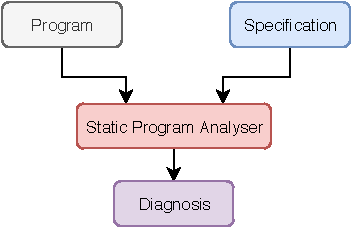
\includegraphics[width=.4 \linewidth]{static_analysis.pdf}
    \caption{%
        Static program analysis~\cite{AIBasedFormalMethodsCousot}
    }
    \label{fig:statAnalysis}
\end{figure}

It is well-known that testing, i.e., executing programs
with some input data and examining the output, may expose errors, but it
can not prove their absence. (It was also famously stated by Edsger W.
Dijkstra: \uv{\textit{Program testing can be used to show the presence of bugs,
but never to show their absence!}}.) However, static program analysis
can prove their absence\,---\,with some \emph{approximation}\,---\,it can
check \emph{all possible executions} of the programs and provide guarantees
about their properties. Another advantage of static analysis is that the
analysis can be performed during the development process, so the program
does not have to be executable yet and it already can be analysed.
The significant issue is how to ensure high precision and
\emph{scalability} to be useful in practice. The biggest disadvantage is
that static analysis can produce many \emph{false alarms}\footnote{%
\textbf{False alarms}\,--\,incorrectly reported an error. Also called
\emph{false positives}.}, but it is often
resolved by accepting \emph{unsoundness}\footnote{\textbf{Soundness}\,--\,if
a~verification method claims that a~system is correct according to a~given
specification, it is truly correct.~\cite{favStaticAnalysis}}.

Various forms of static analysis of programs have been invented, for
instance~\cite{favStaticAnalysis}: bug pattern searching, data-flow
analysis, constraint-based analysis, type analysis, symbolic execution. And
one of the essential concept\,---\,\emph{abstract interpretation}\,---\,is
detailed in Section~\ref{sec:AI}.

There exist numerous tools for static analysis (often proprietary and
difficult to openly evaluate or extend), e.g.: Coverity, Klockwork, CodeSonar,
Loopus, phpstan, or \emph{Facebook Infer} (described in
Section~\ref{sec:fbinfer}).


\subsection{Abstract Interpretation}
\label{sec:AI}

This section explains and defines the basics of \emph{abstract interpretation}.
The description is based on~\cite{AIBasedFormalMethodsCousot},
\cite{AILatticeModelCousot}, \cite{AIInNutshellCousot}, \cite{AICousotWeb},
\cite{favAI}, \cite{projectPracticeMarcin2018}, \cite{wideningNarrowingCousot},
\cite{programAnalysisNielson}, \cite{staticAnalysisMoller},
\cite{favLatticesAndFixpoints}. In these bibliographies, there also can be
found more detailed, more formal, and a~more theoretical explanation.

The abstract interpretation was introduced and formalised by a~French
computer scientist Patrick Cousot and his wife Radhia Cousot in the year
1977 at POPL\footnote{\textbf{POPL}\,--\,symposium on Principles of Programming
Languages.}~\cite{AILatticeModelCousot}. It is a~generic \emph{framework}
for static analyses. It is possible to create particular analyses by
providing specific components (described later) to the framework. The
analysis is guaranteed to be \emph{sound} if certain properties of the
components are met.~\cite{favAI}, \cite{projectPracticeMarcin2018}

In general, in the set theory, which is independent on an application
setting, abstract interpretation is considered theory for
\emph{approximating} sets and set operations. A~more restricted formulation
of abstract interpretation is to interpret it as a~theory of approximation
of the behaviour of the \emph{formal semantics} of programs. Those
behaviours may be characterised by \emph{fixpoints} (defined below), that is
why a~primary part of the theory provides efficient techniques for
\emph{fixpoint approximation}~\cite{programAnalysisNielson}.
So, for a~standard semantics, abstract interpretation is used to derive
the approximate abstract semantics over an \emph{abstract domain} (defined
below), in order to check a~given \emph{program specification} using
analysation of the abstract semantics.~\cite{AIBasedFormalMethodsCousot}

Patrick Cousot intuitively and informally illustrates abstract
interpretation in~\cite{AIInNutshellCousot} as follows.
Figure~\ref{fig:ai1} shows the \emph{concrete semantics} of a~program
by a~set of curves, which represents the set of all possible executions
of the program in all possible execution environments. Each curve shows
the evolution of the vector~$ x(t) $~of input values, state, and
output values of the program as a~function of the time~$ t $.
\emph{Forbidden zones} on this figure represent a~set of erroneous states
of the program execution. Proving, that the intersection of the concrete
semantics of the program with the forbidden zone is empty, is undecidable
because the program concrete semantics is not computable. As demonstrates
Figure~\ref{fig:ai2}, abstract interpretation deals with an
\emph{abstract semantics}, i.e., the \emph{superset} of the concrete
program semantics. The abstract semantics includes all possible executions.
That implies that if the abstract semantics is safe (i.e. does not
intersect the forbidden zone), concrete semantics is safe as well. However,
the \emph{over-approximation} of the possible program executions causes
that inexisting program executions are considered, that may lead to
\emph{false alarms}. It is the case when the abstract semantics
intersects the forbidden zone, whereas the concrete semantics does not
intersect it.

\begin{figure}[hbt]
    \centering

    \begin{subfigure}[hbt]{.45 \linewidth}
        \centering
        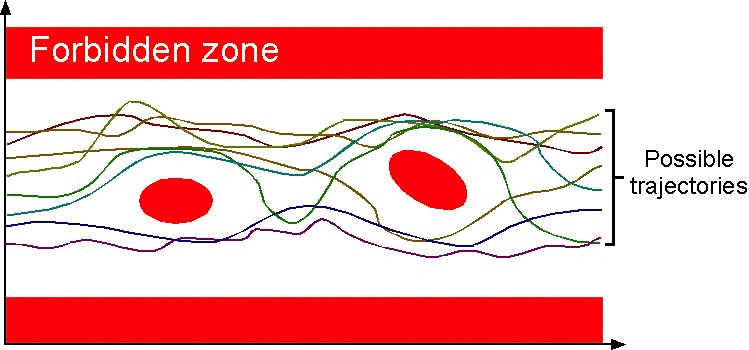
\includegraphics[width=1 \linewidth]{ai_1.png}
        \caption{%
            \emph{Concrete semantics} of programs with
            \emph{forbidden zones}
        }
        \label{fig:ai1}
    \end{subfigure}
%
    \hfill
%
    \begin{subfigure}[hbt]{.45\linewidth}
        \centering
        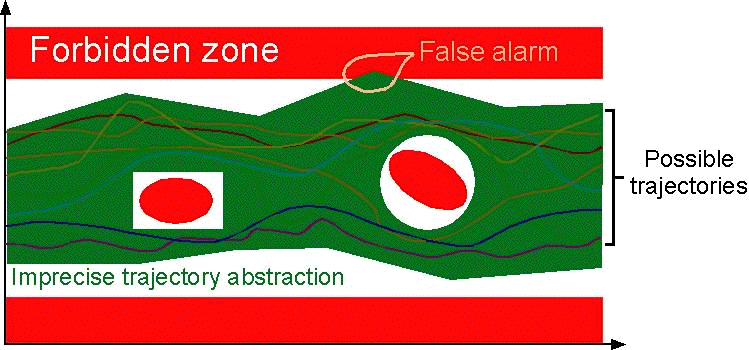
\includegraphics[width=1 \linewidth]{ai_2.png}
        \caption{%
            \emph{Abstract semantics} of programs with imprecise
            trajectory abstraction
        }
        \label{fig:ai2}
    \end{subfigure}

    \caption{%
        Abstract interpretation demonstration~\cite{AIInNutshellCousot}.
        Horizontal axes: time~$ t $. Vertical axes:
        vector~$ x(t) $~of input values of programs
    }
\end{figure}

\subsubsection{Components of Abstract Interpretation}

In accordance with~\cite{favAI}, \cite{projectPracticeMarcin2018},
basic components of abstract interpretation are as follows:
\begin{itemize}
    \item \textbf{Abstract Domain}~\cite{AICousotWeb}
        \begin{itemize}
            \item
                An abstraction of the \emph{concrete semantics} in the form
                of \emph{abstract properties}\footnote{\textbf{Abstract
                properties} approximating \emph{concrete properties
                behaviours}.} and \emph{abstract
                operations}\footnote{\textbf{Abstract operations} include
                abstractions of the \emph{concrete approximation}, an
                approximation of the \emph{concrete fixpoint transform
                function}, etc.}.~\cite{AIBasedFormalMethodsCousot}

            \item
                Sets of program states at certain locations are represented
                using \emph{abstract states}.
        \end{itemize}

    \item \textbf{Abstract Transformers}
        \begin{itemize}
            \item
                There is a~\emph{transform function} for each program
                operation (instruction) that represents the impact
                of the operation executed on an abstract state.
        \end{itemize}

    \item \textbf{Join Operator}~$ \circ $
        \begin{itemize}
            \item
                Joins abstract states from individual program branches into
                a~single one.
        \end{itemize}

    \item
        \textbf{Widening
        Operator~$ \triangledown $}~\cite{programAnalysisNielson},
        \cite{wideningNarrowingCousot}, \cite{favAI}
        \begin{itemize}
            \item
                Enforces termination of the abstract interpretation.

            \item
                It is used to approximate the \emph{least fixed points}
                (it is performed on a~sequence of abstract states at
                a~certain location).

            \item
                The later in the analysis is this operator used, the more
                accurate is the result (but the analysis takes more time).
        \end{itemize}

    \item
        \textbf{Narrowing
        Operator~$ \vartriangle $}~\cite{programAnalysisNielson},
        \cite{wideningNarrowingCousot}, \cite{favAI}
        \begin{itemize}
            \item
                Encapsulates a~termination criterion.

            \item
                Using this operator, the approximation can be refined, i.e.,
                it may be used to refine the result of widening.

            \item
                This operator is used when a~\emph{fixpoint} is
                approximated using widening.
        \end{itemize}
\end{itemize}

\subsubsection{Fixpoints and Fixpoint Approximation}

\begin{definition}
    In~\cite{favLatticesAndFixpoints}, there is a~\emph{fixpoint} defined as:
    \begin{itemize}
        \item
            let $ (A, \leq_A) $ be
            a~\emph{lattice}~\cite{favLatticesAndFixpoints},

        \item
            an element $ a \in A $ is a~\textbf{fixpoint} of a~function
            $ f : A \rightarrow A $ if and only if $ \boldsymbol{f(a) = a} $.
    \end{itemize}
\end{definition}

Computation of the \emph{most precise abstract fixpoint} is not generally
guaranteed to terminate in certain cases, such as loops. The solution is
to approximate the fixpoint using \emph{widening} (over-approximation of
a~fixpoint) and \emph{narrowing} (improves an approximation of
a~fixpoint)~\cite{favAI}, \cite{projectPracticeMarcin2018}.
Most program properties can be represented as fixpoints. This reduces program
analysis to the fixpoint approximation~\cite{AICousotWeb}. Further
information about fixpoint approximation can be found
in~\cite{programAnalysisNielson}, \cite{wideningNarrowingCousot}.

\subsubsection{Formal Definition of Abstract Interpretation}

\begin{definition}
    According to~\cite{AILatticeModelCousot}, \cite{favAI},
    \textbf{abstract interpretation}~$ \boldsymbol{I} $~of a~program~$ P $~with
    the instruction set~$ S $~is a~tuple
    $$ \boldsymbol{I = (Q, \circ, \sqsubseteq, \top, \bot, \tau)} $$
    where
    \begin{itemize}
        \item
            $ \boldsymbol{Q} $~is the \emph{abstract domain} (domain of
            \emph{abstract states}),

        \item
            $ \boldsymbol{\circ}~\text{:}~Q \times Q \rightarrow Q $
            is the \emph{join operator} for accumulation of abstract states,

        \item
            $ \text{(}\boldsymbol{\sqsubseteq}\text{)} \subseteq Q \times Q $ is
            \emph{ordering} defined as
            $ x \sqsubseteq y \Leftrightarrow x \circ y = y $ in
            $ (Q, \circ, \top) $,

        \item
            $ \boldsymbol{\top} \in Q $ is a~\emph{supremum} of~$ Q $,

        \item
            $ \boldsymbol{\bot} \in Q $ is an \emph{infimum} of~$ Q $,

        \item
            $ \boldsymbol{\tau}~\text{:}~S \times Q \rightarrow Q $
            defines the \emph{abstract transformers} for specific instructions,

        \item
            $ (Q, \circ, \top) $ is a~\emph{complete
            semilattice}~\cite{favLatticesAndFixpoints}, \cite{favAI}.
    \end{itemize}
\end{definition}

Using so-called \emph{Galois connections}~(\cite{programAnalysisNielson},
\cite{wideningNarrowingCousot}, \cite{favAI}, \cite{AICousotWeb}) can be
guaranteed the \emph{soundness} of abstract interpretation.


\section{\texorpdfstring{Facebook Infer\,--\,Static Analysis Framework}{}}
\label{sec:fbinfer}

This section describes the principles and features of
\emph{Facebook Infer}. The description is based on information provided
on Facebook Infer website\footnote{\textbf{Facebook Infer}
website\,--\,\url{https://fbinfer.com}.} and in~\cite{inferAISlides},
\cite{projectPracticeMarcin2018}. Parts of this section are taken
over~\cite{excel2019FBInfer}.

Facebook Infer is an open-source\footnote{\textbf{Open-source repository of
Facebook Infer} on GitHub\,--\,\url{https://github.com/facebook/infer}.}
static analysis \emph{framework},which is able to discover various kinds of
software bugs of a~given program, and the stress is put on \emph{scalability}.
Elementary essence of this framework shows Figure~\ref{fig:infer}, below
is a~more detailed explanation of its architecture. Facebook Infer
itself is implemented in \emph{OCaml}\footnote{\textbf{OCaml}
website\,--\,\url{https://ocaml.org}.}\,--\,\emph{functional} programming
language, also supporting \emph{imperative} and \emph{object-oriented}
paradigms. Further details about OCaml can be found in~\cite{realWorldOCaml}
or in official documentation\footnote{\textbf{OCaml
documentation}\,--\,\url{http://caml.inria.fr/pub/docs/manual-ocaml}.},
tutorials\footnote{\textbf{OCaml
tutorials}\,--\,\url{https://ocaml.org/learn/tutorials}.}. Facebook Infer was
originally a~standalone tool focused on \emph{sound verification} of
the absence of \emph{memory safety violations}, which has made its breakthrough
thanks to a~powerful paper~\cite{inferBiabduction}.

\begin{figure}[hbt]
    \centering
    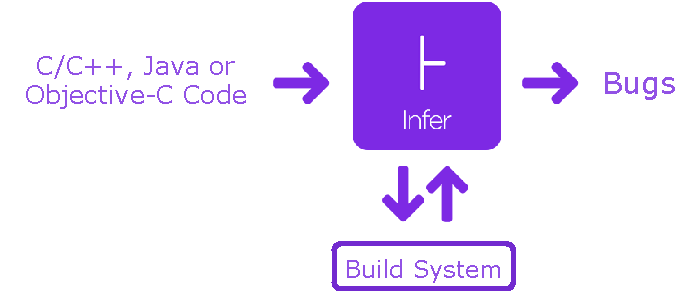
\includegraphics[width=.7 \linewidth]{infer.pdf}
    \caption{%
        Static analysis in Facebook Infer
        (\url{%
            http://www.codeandyou.com/2015/06/%
            infer-static-analyzer-for-java-c-and.html%
        })
    }
    \label{fig:infer}
\end{figure}

Facebook Infer is able to analyse programs written in several languages.
In particular, it supports languages C, C++, Java, and Objective-C. Moreover,
it is possible to extend Facebook Infer's \emph{frontend} for supporting
another languages. Currently, Facebook Infer contains many analyses focusing
on amount sorts of bugs, e.g., \emph{Inferbo} (buffer
overruns)~\cite{inferboOnline}; \emph{RacerD} (data races)~\cite{racerD},
\cite{racerDOnline}, \cite{staticRaceDetectorTruePositive}; and other analyses
checks for buffer overflows, thread-safety, null-dereferencing, memory leaks,
resource leaks, etc.


\subsection{Abstract Interpretation in Facebook Infer}
\label{sec:fbinferAI}

Facebook Infer is a~general framework for static analysis of programs, it is
based on \emph{abstract interpretation}, see Section~\ref{sec:AI}. It aims
to find bugs rather than formal verification. It can be used to quickly develop
new sorts of \emph{compositional} and \emph{incremental} analysers
(\emph{intraprocedural} or
\emph{interprocedural}~\cite{programAnalysisNielson}) based
on the concept of function \emph{summaries}. In general, a~\emph{summary}
is a~representation of \emph{preconditions} and \emph{postconditions} of
a~function. However, in practice, a~summary is a~custom data structure that
may be used for storing any information resulting from the analysis of
single functions. Facebook Infer generally does not work out the summaries
in the course of the analysis along the \emph{Control Flow Graph}
(\textbf{CFG})\footnote{\textbf{A~control flow graph (CFG)} is a~directed
graph in which the nodes represent basic blocks and the edges represent control
flow paths.~\cite{controlFlowAnalysisAllen}} as it is done in classical
analyses based on the concepts from~\cite{dataflowAnalysisGraphReachability},
\cite{dataflowAnalysisApproaches}. Instead, Facebook Infer performs the
analysis of a~program \emph{function-by-function along the call tree},
starting from its leafs (demonstrated later). Therefore a~function
is analysed and a~summary is computed without knowledge of the
call context. Since summaries worked out in different contexts are equal,
this principle makes the analysis more scalable, but it can lead to
a~loss of accuracy. Then, the summary of a~function is used at all of its
call sites. In order to create new intraprocedural analyser in Facebook
Infer, it is needed to define (listed items are described in more detail
in Section~\ref{sec:AI}):
\begin{enumerate}
    \item
        The \emph{abstract domain}~$ Q $, i.e., a~type of an
        \emph{abstract state}.

    \item
        Operator~$ \sqsubseteq $, i.e., \emph{ordering} of abstract
        states.

    \item
        The \emph{join} operator~$ \circ $, i.e., the way of joining two
        abstract states.

    \item
        The \emph{widening} operator~$ \triangledown $, i.e., the way how to
        enforce termination of the abstract interpretation of iteration.

    \item
        \emph{Transfer functions}~$ \tau $, i.e., a~transformer that
        takes an abstract state as an input and produces an abstract state
        as an output.
\end{enumerate}
And in order to create an interprocedural analyser, it is required to
additionally define:
\begin{enumerate}
    \item
        A~type of function summaries.

    \item
        The logic for using summaries in transfer functions, and the logic
        for transforming an intraprocedural abstract state to
        a~summary.
\end{enumerate}
The next important feature improving the scalability is
\emph{incrementality} of the analysis, it allows to analyse separate
code changes only, instead of analysing the whole codebase. It is more
suitable for extensive and variable projects, where ordinary analysis
is not feasible. The incrementality is based on \emph{re-using summaries}
of functions for which there is no change in them neither in the functions
transitively invoked from them.

\subsubsection{%
    The Architecture of the Abstract Interpretation Framework in
    Facebook Infer
}

The architecture of the abstract interpretation framework of Facebook
Infer (\textbf{Infer.AI}) may be split into three major parts,
as demonstrates Figure~\ref{fig:inferArch}: a~\emph{frontend},
an \emph{analysis scheduler} (and a~\emph{results database}), and a~set of
\emph{analyser plugins}.

\begin{figure}[hbt]
    \centering
    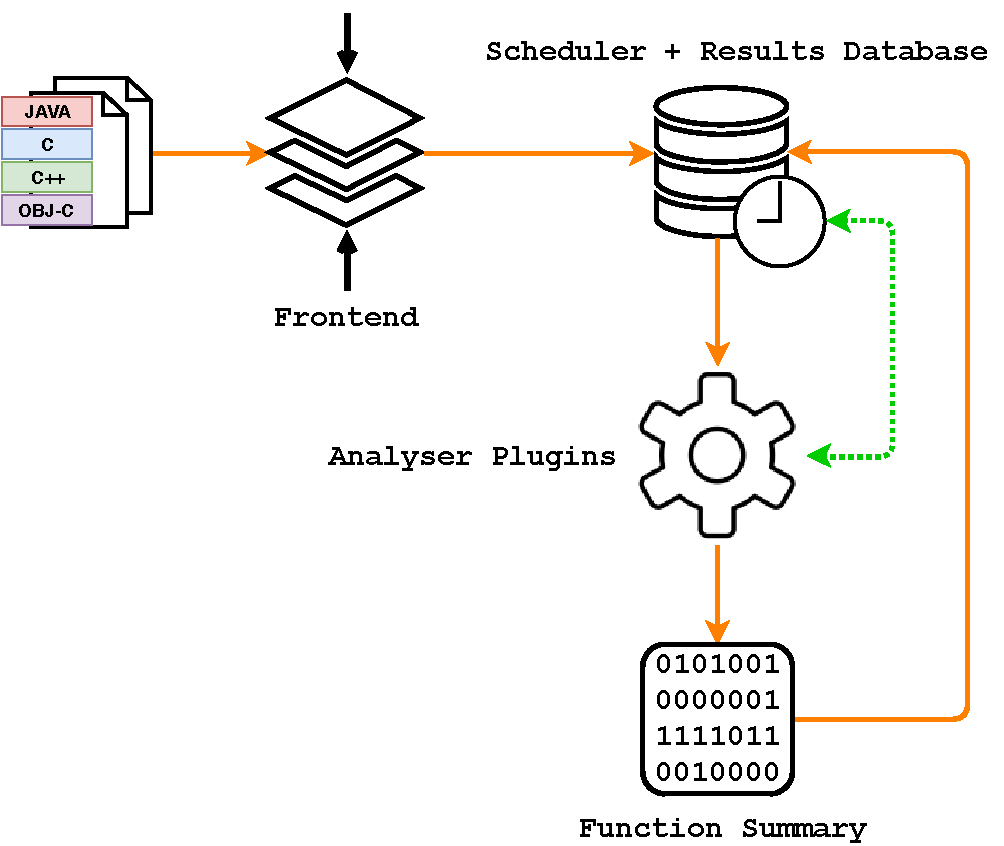
\includegraphics[width=.65 \linewidth]{infer_architecture.pdf}
    \caption{%
        The architecture of Facebook Infer's abstract interpretation
        framework~\cite{inferAISlides}, \cite{projectPracticeMarcin2018}
    }
    \label{fig:inferArch}
\end{figure}

The frontend compiles input programs into the \emph{Smallfoot Intermediate
Language} (SIL) and represents them as the CFG. There is a~separate CFG
representation for each analysed function. Nodes of this CFG are formed as
instructions of SIL. SIL language consists of following underlying
instructions:
\begin{enumerate}
    \item
        \texttt{LOAD}\,--\,reading into a~temporary variable.

    \item
        \texttt{STORE}\,--\,writing to a~program variable,
        a~field of a~structure, or an array.

    \item
        \texttt{PRUNE~e}~(often called
        \texttt{ASSUME})\,--\,a~condition~\texttt{e}.

    \item
        \texttt{CALL}\,--\,a~function call.
\end{enumerate}
The frontend allows one to propose \emph{language-independent} analyses
(to a~certain extent) because it supports input programs to be written
in multiple languages.

The next part of the architecture is the scheduler, which defines the
order of the analysis of single functions according to the appropriate
\emph{call graph}\footnote{\textbf{A~call graph} is \emph{directed graph}
describing call dependencies among functions.}. The scheduler also checks
\begin{wrapfigure}{r}{.45 \linewidth}
    \centering
    \vspace{-.5em}
    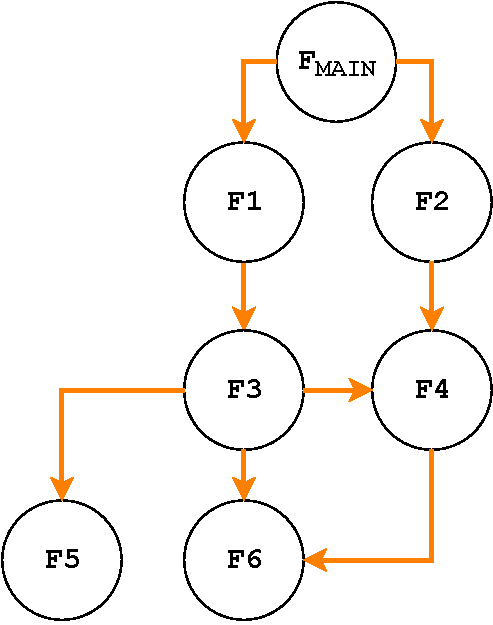
\includegraphics[width=.23 \textwidth]{infer_call_graph.pdf}
    \caption{%
        A~call graph for an illustration of Facebook Infer's
        analysis process~\cite{inferAISlides}, \cite{excel2019FBInfer},
        \cite{projectPracticeMarcin2018}
    }
    \label{fig:inferCallGraph}
\end{wrapfigure}
if it is possible to analyse some functions simultaneously, which allows
Facebook Infer to run the analysis in parallel.

\begin{example}
    For demonstrating the order of the analysis in Facebook Infer and its
    incrementality, assume a~call graph in Figure~\ref{fig:inferCallGraph}.
    At first, leaf functions \texttt{F5} and \texttt{F6} are analysed. Further,
    the analysis goes on towards the root of the call
    graph\,--\,\texttt{F\textsubscript{MAIN}}, while takes into consideration
    the dependencies denotes by the edges. This order ensures that a~summary
    is available once a~nested function call is abstractly interpreted within
    the analysis. When there is a~subsequent code change, only directly changed
    functions and all the functions up the call path are re-analysed. For
    instance, if there is a~change of source code of function \texttt{F4},
    Facebook Infer triggers re-analysation of functions \texttt{F4},
    \texttt{F2}, and \texttt{F\textsubscript{MAIN}} only.
\end{example}

The last part of the architecture consists of a~set of analyser plugins.
Each plugin performs the analysis by interpretation of SIL instructions.
Result of the analysis of each function (function summary) is stored to
the results database. Interpretation of SIL instructions (\emph{commands})
is done using an \emph{abstract interpreter} (also called a~\emph{control
interpreter}) and \emph{transfer functions} (also called a~\emph{command
interpreter}). The transfer functions take an actual \emph{abstract state}
of an analysed function as an input, and by applying the interpreting command
produce a~new abstract state. Then, the abstract interpreter interprets the
command in \emph{abstract domain} according to the CFG. This workflow is
simplified in Figure~\ref{fig:inferAnalysis}.

\begin{figure}[hbt]
    \centering
    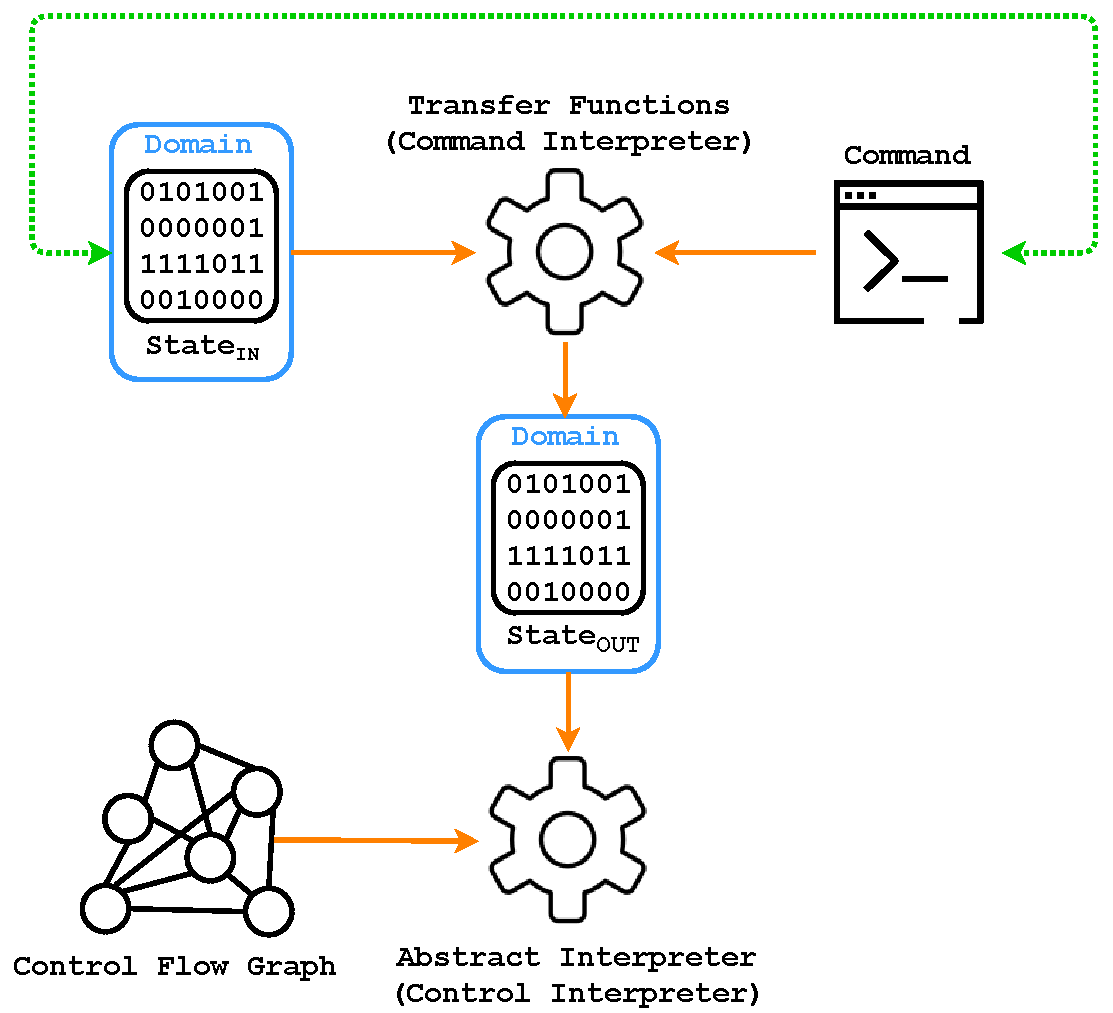
\includegraphics[width=.65 \linewidth]{infer_analysis.pdf}
    \caption{%
        Facebook Infer's abstract interpretation
        process~\cite{inferAISlides}, \cite{projectPracticeMarcin2018}
    }
    \label{fig:inferAnalysis}
\end{figure}


\section{Contracts for Concurrency}
\label{sec:contracts}

This section introduces and defines the concept of \emph{contracts for
concurrency} described in~\cite{contracts2015}, \cite{contracts2017}. Parts
of this section are taken over~\cite{excel2019FBInfer}. Listings in this
section are pieces of programs written in ANSI~C\footnote{%
\textbf{ANSI~C}\,--\,standard for the C~programming language published by
the \emph{ANSI} (American National Standards Institute).}.

Respecting the \emph{protocol} of a~software module\,---\,delineates
which \emph{sequences of functions} are legal to invoke\,---\,is one of the
requirements for the correct behaviour of the module. For example, a~module
that deals with file system typically requires that a~programmer using
this module should call function \texttt{open} at first, followed by an
optional number of functions \texttt{read} and \texttt{write}, and at last,
call function \texttt{close}. A~program utilising such a~module that does
not follow this protocol is erroneous. The methodology of \emph{design by
contract} (described in~\cite{contract}) requires programs to meet
such well-defined behaviours.~\cite{contracts2015}

In \emph{concurrent programs}, contracts for concurrency allow one to specify
\emph{sequences of functions} that are needed to be \emph{executed
atomically}, in order to avoid \emph{atomicity violations}. Such contracts
may be manually specified by a~developer or it may be automatically generated
by a~program (analyser). These contracts can be used to verify the correctness
of programs as well as they can serve as helpful documentation. A~program is
safe from atomicity violations if the program follows the contract and
the contract is well-defined and complete.

Section~\ref{sec:basicContracts} defines the notion of \emph{basic contracts
for concurrency}. Further, Section~\ref{sec:paramContracts} defines
contracts extended to consider the \emph{data flow} between functions (i.e.,
a~sequence of function calls must be atomic only if they handle the
same data). Above that, paper~\cite{contracts2017} extends the idea
of basic contracts with \emph{spoilers} (i.e., extending by
\emph{contextual information}).


\subsection{Basic Contracts}
\label{sec:basicContracts}

\begin{definition}
    In~\cite{contracts2017}, \cite{contracts2015}, a~\emph{basic contract} is
    formally defined as follows. Let~$ \Sigma_\mathbb{M} $~be a~set of all
    function names of a~software module. A~contract is
    a~set~$ \mathbb{R} $~of \emph{clauses} where each clause
    $ \varrho\ \in \mathbb{R} $ is a~\emph{star-free regular
    expression}\footnote{\textbf{Star-free regular expressions} are
    regular expressions using only the \emph{concatenation operators}
    and the \emph{alternative operators} ($ | $), without the
    \emph{Kleene star operator} ($ * $).} over~$ \Sigma_\mathbb{M} $.
    A~\emph{contract violation} occurs if any of the sequences expressed by
    the contract clauses are interleaved with the execution of functions
    from~$ \Sigma_\mathbb{M} $, in other words, each sequence specified by
    any clause~$ \varrho $~must be executed atomically, otherwise, there
    is a~violation of the contract. The number of sequences defined by
    a~contract is finite since the contract is the union of
    \emph{star-free languages}.
\end{definition}

\begin{example}
    Consider the following example from~\cite{contracts2017},
    \cite{contracts2015}. There is a~module with the implementation of
    a~resizable array with the listed functions:
    \begin{enumerate}[label={$ f_{\arabic*} $:}]
        \tt

        \item
            \textcolor{bluekeywords}{void} add(%
                \textcolor{bluekeywords}{char} *array,
                \textcolor{bluekeywords}{char} element%
            )

        \item
            \textcolor{bluekeywords}{bool} contains(%
                \textcolor{bluekeywords}{char} *array,
                \textcolor{bluekeywords}{char} element%
            )

        \item
            \textcolor{bluekeywords}{int} index\_of(%
                \textcolor{bluekeywords}{char} *array,
                \textcolor{bluekeywords}{char} element%
            )

        \item
            \textcolor{bluekeywords}{char} get(%
                \textcolor{bluekeywords}{char} *array,
                \textcolor{bluekeywords}{int} index%
            )

        \item
            \textcolor{bluekeywords}{void} set(%
                \textcolor{bluekeywords}{char} *array,
                \textcolor{bluekeywords}{int} index,
                \textcolor{bluekeywords}{char} element%
            )

        \item
            \textcolor{bluekeywords}{void} remove(%
                \textcolor{bluekeywords}{char} *array,
                \textcolor{bluekeywords}{int} index%
            )

        \item
            \textcolor{bluekeywords}{int} size(%
                \textcolor{bluekeywords}{char} *array%
            )
    \end{enumerate}
    The module's contract contains the following clauses:
    \begin{enumerate}[label={$ (\varrho_{\arabic*}) $}]
        \item
            \texttt{contains index\_of}
            \begin{itemize}[label=]
                \item
                    The execution of \texttt{contains} followed by the execution
                    of \texttt{index\_of} should be atomic. Otherwise,
                    the program may fail to get the index, because after
                    verification of the presence of an element in an array, it
                    can be concurrently, e.g., removed.
            \end{itemize}

        \item
            \texttt{index\_of (get | set | remove)}
            \begin{itemize}[label=]
                \item
                    The execution of \texttt{index\_of} follow by the execution
                    of \texttt{get}, \texttt{set}, or \texttt{remove} should be
                    atomic. Otherwise, the received index may be outdated when
                    it is applied to address an element, because a~concurrent
                    modification of
                    an array may shift the position of the element.
            \end{itemize}

        \item
            \texttt{size (get | set | remove)}
            \begin{itemize}[label=]
                \item
                    The execution of \texttt{size} followed by the execution of
                    \texttt{get}, \texttt{set}, or \texttt{remove} should be
                    atomic. Otherwise, the size of an array may be void when
                    accessing an array, because of a~concurrent change of the
                    array. This can be an issue since a~given index is not in
                    a~valid range anymore (e.g., testing \texttt{index < size}).
            \end{itemize}

        \item
            \texttt{add (get | index\_of)}
            \begin{itemize}[label=]
                \item
                    The execution of \texttt{add} followed by the execution of
                    \texttt{get} or \texttt{index\_of} should be atomic.
                    Otherwise, the added element does not have to longer exist
                    or its position in an array can be changed, when the program
                    attempts to obtain information about it.
            \end{itemize}
    \end{enumerate}
\end{example}

The above definition of contracts for concurrency is quite limited in
some circumstances and can consider valid concurrent programs as erroneous
(reports \emph{false alarms}). Hence, in Section~\ref{sec:paramContracts},
there is defined an extension of contracts for concurrency with
\emph{parameters}, which takes into consideration the data flow within
function calls. And in~\cite{contracts2017}, \cite{contracts2015}, there is
defined another extension with \emph{spoilers}, which considering contextual
information of function calls.


\subsection{Contracts with Parameters}
\label{sec:paramContracts}

\begin{example}
    Consider the following example from~\cite{contracts2017},
    \cite{contracts2015}, as demonstrates Listing~\ref{list:contractsReplace}.
    There is a~function \texttt{replace} that replaces item~\texttt{a}~in an
    array by item~\texttt{b}. Implementation of this function comprises two
    atomicity violations:
    \begin{enumerate}[label={(\roman*)}]
        \item
            when \texttt{index\_of} is invoked, item~\texttt{a}~does not need to
            be in the array anymore;

        \item
            the acquired index can be obsolete when \texttt{set} is invoked.
    \end{enumerate}
    A~basic contract defined in Section~\ref{sec:basicContracts} could cover
    this scenario by clause~$ \varrho_5 $:
    $$ (\varrho_5)\ \text{\texttt{contains index\_of set}} $$
    Nevertheless, it is too restrictive because it is required to be executed
    atomically only if \texttt{contains} and \texttt{index\_of} have the same
    arguments \texttt{array} and \texttt{element}, \texttt{index\_of} and
    \texttt{set} have the same argument \texttt{array}, and the returned value
    of \texttt{index\_of} is used as the argument \texttt{index} of function
    \texttt{set}.
\end{example}

\begin{lstlisting}[
    style=c, label={list:contractsReplace}, float=hbt,
    caption={%
        An example of an atomicity violation with data
        dependencies~\cite{contracts2017}
    }
]
void replace(char *array, char a, char b)
{
    if (contains(array, a))
    {
        int index = index_of(array, a);
        set(array, index, b);
    }
}
\end{lstlisting}

In order to respect function call \emph{parameters} and \emph{return values}
of functions in contracts, the basic contracts are further extended by
dependencies among functions in~\cite{contracts2017}, \cite{contracts2015}
as follows. Function call parameters and return values are expressed as
\emph{meta-variables}. Further, if a~contract should be required exclusively
if the same object emerges as an argument or as the return value of multiple
calls in a~given call sequence, it may be denoted by using the same
meta-variable at the position of all these occurrences of parameters and
return values.

Clause~$ \varrho_5 $~can be extended as follows (repeated application of
meta-variables \texttt{X/Y/Z} requiring the same objects
\texttt{o\textsubscript{1}/o\textsubscript{2}/o\textsubscript{3}} to be used
at the positions of \texttt{X/Y/Z}):
$$
    (\varrho^\prime_5)\ \text{\texttt{%
        contains(X,Y) Z=index\_of(X,Y) set(X,Z,\_)
    }}
$$
The underscore indicates a~\emph{free meta-variable} that does not restrict
the contract clause.

With the extension described above, it is possible to extend the contract
from Section~\ref{sec:basicContracts} as follows:
\begin{enumerate}[label={$ (\varrho^\prime_{\arabic*}) $}]
    \tt

    \item contains(X,Y) index\_of(X,Y)
    \item Y=index\_of(X,\_) (get(X,Y) | set(X,Y,\_) | remove(X,Y))
\end{enumerate}



\chapter{Proposal of Static Analyser for Detecting Atomicity Violations}
\label{chap:proposal}

This chapter describes a~proposal of a~static program analyser for
detection of \emph{atomicity violations}. The proposed
analyser\,---\,\textbf{Atomer}\,---\,has been proposed as an extension
for \emph{Facebook Infer}, introduced in Section~\ref{sec:fbinfer}. In
particular, the proposal concentrates on an \emph{atomic execution of
sequences of function calls}, which is often required. The
proposed principle is based on the assumption that sequences executed
\emph{once atomically} should probably be executed \emph{always atomically}.
The chapter also assessments already existing solutions in this area.

At first, Section~\ref{sec:existAnalysers} deals with
existing approaches and tools for finding atomicity violations, their
advantages, disadvantages, features, availability, and so on. Then,
the proposal itself is introduced in Section~\ref{sec:proposal}. Parts of
this chapter are taken over~\cite{excel2019FBInfer}. Listings in this
chapter are pieces of exemplary programs written in ANSI~C (assume
\emph{PThread} locks and the existence of an initialised global variable
\texttt{lock} of a~type \texttt{pthread\_mutex\_t}).


\section{Assessment of Existing Analysers for Atomicity-Related Errors}
\label{sec:existAnalysers}

The proposed solution is slightly inspired by ideas from~\cite{contracts2017},
\cite{contracts2015}. In these papers, there is described a~proposal
and implementation of a~\emph{static validation} for finding
\emph{atomicity violations}, which is based on \emph{grammars} and
\emph{parsing trees}. In paper~\cite{contracts2017}, there is also described
and implemented a~dynamic approach to this validation. The authors
of~\cite{contracts2017} and~\cite{contracts2015} implemented a~stand-alone
prototype tool\footnote{\textbf{Gluon}\,---\,a~tool for static verification of
\emph{contracts for concurrency} (see Section~\ref{sec:contracts}) in Java
programs\,---\,\url{https://github.com/trxsys/gluon}.} for analysing programs
written in Java. It led to some promising experimental results but the
\emph{scalability} of the tool was still limited. Moreover, the tool
from~\cite{contracts2017} and~\cite{contracts2015} is no more developed. That
is why was made the decision to get inspired by~\cite{contracts2017}
and~\cite{contracts2015} and reimplement the analysis in \emph{Facebook Infer}
redesigning it in accordance with the principles of Facebook Infer (described in
Section~\ref{sec:fbinfer}), which should make it more scalable. In the end, due
to adapting the analysis for the context of Facebook Infer, implementation of
the analysis within this thesis is significantly different
from~\cite{contracts2017} and~\cite{contracts2015}, as it is presented in
Chapter~\ref{chap:implementExp}. Furthermore, unlike~\cite{contracts2017}
and~\cite{contracts2015}, the implementation aims at programs written
in C/C++ languages using \emph{POSIX Thread (PThread)} locks for
a~\emph{synchronisation of concurrent threads}.

In Facebook Infer, there is already implemented analysis called
\emph{Lock Consistency Violation}\footnote{\textbf{Lock Consistency
Violation}\,---\,atomicity violations analysis in Facebook
Infer\,---\,\url{https://fbinfer.com/docs/%
checkers-bug-types.html\#LOCK_CONSISTENCY_VIOLATION}.}. It is part of
\emph{RacerD}~\cite{racerD}, \cite{racerDOnline},
\cite{staticRaceDetectorTruePositive}. This analysis finds atomicity
violations for writes/reads on single variables that are required to
be executed atomically. Atomer is different, it finds atomicity
violations for \emph{sequences of functions} that are required to be
executed atomically, i.e., it checks whether \emph{contracts for
concurrency} (see Section~\ref{sec:contracts}) hold.


\section{Proposal of the Analyser}
\label{sec:proposal}

The proposal of the analyser is based on the concept of \emph{contracts
for concurrency} described in Section~\ref{sec:contracts}. In particular,
the proposal considers only \emph{basic contracts} described in
Section~\ref{sec:basicContracts}. Parameters of functions and their
return values\,---\,expressed in \emph{contracts with parameters}
(see Section~\ref{sec:paramContracts})\,---\,are not taken into
consideration.

In general, basic contracts for concurrency allow one to define
\emph{sequences of functions} that are required to be \emph{executed
atomically}, as it is explained in more detail in Section~\ref{sec:contracts}.
Atomer is able to automatically derive candidates for such contracts, and
then to verify whether the contracts are fulfilled. Both of these operations
are done statically. The proposed analysis is divided into two parts
(\emph{phases of the analysis}):
\begin{enumerate}[label={\textbf{Phase \arabic*}:}, leftmargin=6em]
    \item
        Detection of \emph{atomic sequences}, which is described in
        Section~\ref{sec:proposalPhase1}.

    \item
        Detection of \emph{atomicity violations} (violations of the atomic
        sequences), which is described in Section~\ref{sec:proposalPhase2}.
\end{enumerate}
These phases of the analysis and its workflow illustrate
Figure~\ref{fig:analyserPhases}.

\begin{figure}[hbt]
    \centering
    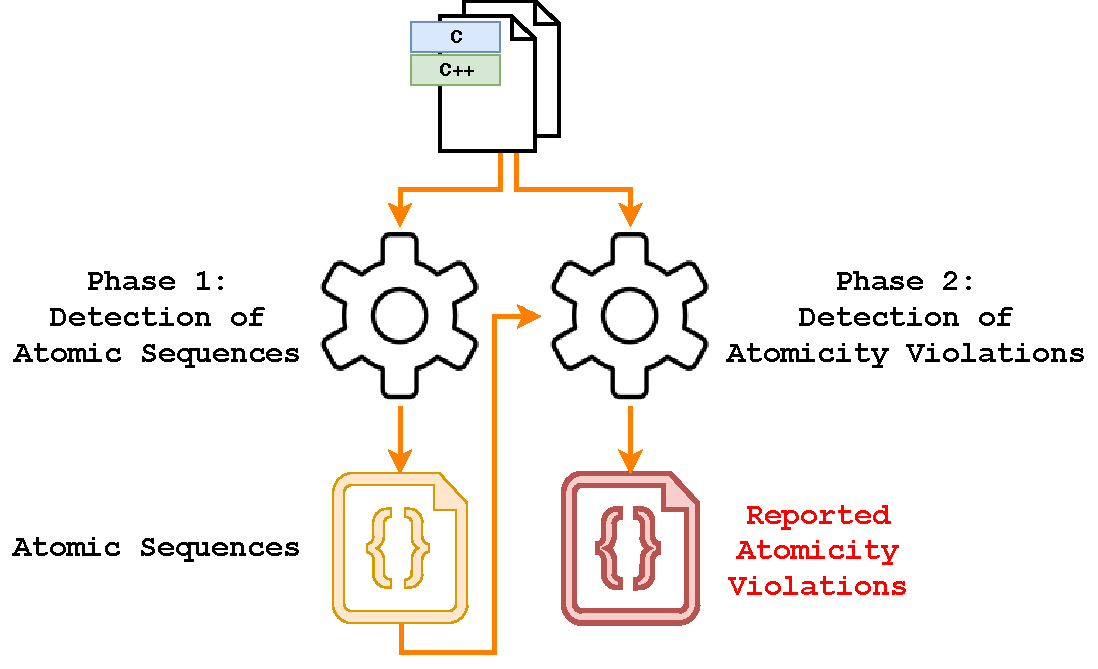
\includegraphics[width=.75 \linewidth]{analyser_proposal.pdf}
    \caption{Phases of the proposed analyser}
    \label{fig:analyserPhases}
\end{figure}


\subsection{Phase 1: Detection of Atomic Sequences}
\label{sec:proposalPhase1}

Before the detection of \emph{atomicity violations}
(Section~\ref{sec:proposalPhase2}) may begin, it is required to have
contracts introduced in Section~\ref{sec:contracts}. \textbf{Phase 1}
of Atomer is able to produce such contracts, i.e., it detects
\emph{sequences of functions} that should be \emph{executed atomically}.
Intuitively, the detection is based on looking for sequences of
functions that are executed atomically on some path through
a~program. The assumption is that if it is once needed to execute
a~sequence atomically, it should probably be always executed atomically.

The detection of sequences of calls to be executed atomically is based on
analysing all paths through the CFG of a~function and generating all
pairs~\textbf{(A,~B)} of sets of function calls such that: \textbf{A}~is
a~\emph{reduced sequence} of function calls that appear between the
beginning of the function being analysed and the first lock or between an
unlock and a~subsequent lock (or between an unlock and the end of the function
being analysed), and \textbf{B}~is a~reduced sequence of function calls that
follow the calls from~\textbf{A}~and that appear between a~lock and an unlock
(or between a~lock and the end of the function being analysed). Here, by
a~reduced sequence, it is meant a~sequence in which the first appearance
of each function is recorded only. The reason is to ensure \emph{finiteness}
of the sequences and of the analysis. The \emph{summary} of a~function
then consists of:
\begin{enumerate}[label={(\roman*)}]
    \item
        the set of all the~\textbf{B}~sequences and

    \item
        the set of \emph{concatenations} of all
        the~\textbf{A}~and \textbf{B}~sequences with the removal of
        duplicate function calls.
\end{enumerate}
The latter is recorded for the purpose of analysing functions higher in the
\emph{call hierarchy} since locks/unlocks can appear in such
a~\emph{higher-level function}.

\begin{example}
    For instance, the analysis of the function~\texttt{g}~from
    Listing~\ref{list:analyserPhase1} produces the following sequences:
    $$
        \overbrace{%
            \text{\texttt{f1}~\sout{\texttt{f1}}}
        }^\text{\textbf{A\textsubscript{1}}}
        \overbrace{%
            (\text{\texttt{f1}~\sout{\texttt{f1}}~\texttt{f2}})
        }^\text{\textbf{B\textsubscript{1}}} |
        \overbrace{%
            \text{\texttt{f1}~\sout{\texttt{f1}}}
        }^\text{\textbf{A\textsubscript{2}}}
        \overbrace{%
            (\text{\texttt{f1}~\texttt{f3}})
        }^\text{\textbf{B\textsubscript{2}}} |
        \overbrace{%
            \text{\sout{\texttt{f1}}}
        }^\text{\sout{\textbf{A\textsubscript{3}}}}
        \overbrace{%
            (\text{\sout{\texttt{f1}~\texttt{f3}~\texttt{f3}}})
        }^\text{\sout{\textbf{B\textsubscript{3}}}}
    $$
    The parentheses are used to indicate an atomic sequence. The
    strikethrough of the functions~\texttt{f1} and \texttt{f3} denotes
    the removal of already recorded function calls in
    the~\textbf{A}~and \textbf{B}~sequences. The strikethrough of the
    entire sequence~\texttt{f1}~(\texttt{f1}~\texttt{f3}~\texttt{f3})
    means discarding sequences already seen before. The derived sets for
    the function~\texttt{g}~are then as follows:
    \begin{enumerate}[label={(\roman*)}]
        \item
           \{(\texttt{f1}~\texttt{f2}),~(\texttt{f1}~\texttt{f3})\}, i.e.,
           \textbf{B\textsubscript{1}}~and \textbf{B\textsubscript{2}};

        \item
            \{\texttt{f1}~\texttt{f2}~\texttt{f3}\}, i.e.,
            concatenation of~\textbf{A\textsubscript{1}},
            \textbf{B\textsubscript{1}}, \textbf{A\textsubscript{2}},
            and \textbf{B\textsubscript{2}} with the removal of duplicate
            function calls.

    \end{enumerate}
\end{example}

\begin{lstlisting}[
    style=c, label={list:analyserPhase1}, float=hbt,
    caption={%
        An example of a~code for an illustration of the derivation of
        sequences of functions called atomically
    }
]
void g(void)
{
    f1(); f1();

    <@\textcolor{red}{pthread\_mutex\_lock}@>(&lock);
    f1(); f1(); f2();
    <@\textcolor{red}{pthread\_mutex\_unlock}@>(&lock);

    f1(); f1();

    <@\textcolor{red}{pthread\_mutex\_lock}@>(&lock);
    f1(); f3();
    <@\textcolor{red}{pthread\_mutex\_unlock}@>(&lock);

    f1();

    <@\textcolor{red}{pthread\_mutex\_lock}@>(&lock);
    f1(); f3(); f3();
    <@\textcolor{red}{pthread\_mutex\_unlock}@>(&lock);
}
\end{lstlisting}

\subsubsection{%
    Analysing Functions Using Results of the Analysis of Nested Functions
}

Further, it is demonstrated how the results of the analysis of \emph{nested
functions} are used during the detection of atomic sequences. The
result of the analysis of a~nested function is used as follows. When
calling an already analysed function, one plugs all the sequences from the
second component of its summary into the
current~\textbf{A}~or~\textbf{B}~sequence.

\begin{example}
    This example shows how the function~\texttt{h}~from
    Listing~\ref{list:analyserPhase1Nested} would be analysed using the
    result of the analysis of the function~\texttt{g}~from
    Listing~\ref{list:analyserPhase1}. So the analysis of the
    function~\texttt{h}~produces the following sequence:
    $$
        \text{%
            \texttt{f1}~\texttt{g}~\sout{\texttt{f1}}~\texttt{f2}~\texttt{f3}
        }
        (\text{%
            \texttt{g}~\texttt{f1}~\texttt{f2}~\texttt{f3}%
        })
    $$
    The derived sets for the function~\texttt{h}~are then as follows:
    \begin{enumerate}[label={(\roman*)}]
        \item
            \{(\texttt{g}~\texttt{f1}~\texttt{f2}~\texttt{f3})\};

        \item
            \{\texttt{f1}~\texttt{g}~\texttt{f2}~\texttt{f3}\}.
    \end{enumerate}
\end{example}

\begin{lstlisting}[
    style=c, label={list:analyserPhase1Nested}, float=hbt,
    caption={%
        An example of a~code for an illustration of the derivation of
        sequences of functions called atomically with a~nested function
        call (function~\texttt{g} is defined in
        Listing~\ref{list:analyserPhase1})
    }
]
void h(void)
{
    f1(); g();

    <@\textcolor{red}{pthread\_mutex\_lock}@>(&lock);
    g();
    <@\textcolor{red}{pthread\_mutex\_unlock}@>(&lock);
}
\end{lstlisting}

\subsubsection{Cases Where Lock/Unlock Calls Are Not Paired in a~Function}

For treating cases where lock/unlock calls are \emph{not paired} in
a~function\,---\,as demonstrates
Listing~\ref{list:analyserPhase1NotPairedLock}\,---\,two solutions
have been proposed:
\begin{enumerate}
    \item
        At the end of a~function, everything is unlocked, i.e., append
        an unlock to the end of the function if it is necessary. Then
        for the function~\texttt{x}~from
        Listing~\ref{list:analyserPhase1NotPairedLock}, the first component
        of its summary (i.e., atomic sequences) would be \{(\texttt{a})\}.
        Subsequently, all unlock calls not preceded by a~lock are
        ignored. So the first component of a~summary of the
        function~\texttt{y}~from
        Listing~\ref{list:analyserPhase1NotPairedLock} would be an empty set.

    \item
        Addition of two further items to the summaries:
        \begin{enumerate}[label={(\alph*)}]
            \item
                function calls with missing an unlock call,

            \item
                function calls with missing a~lock call.
        \end{enumerate}
        For the example from Listing~\ref{list:analyserPhase1NotPairedLock},
        this would give:
        \begin{itemize}
            \item
                for~\texttt{x}:~\{(\texttt{f1}\},

            \item
                for~\texttt{y}:~\{\texttt{f2})\}.
        \end{itemize}
        The above sequences would have to be glued to the sequences
        captured higher in the call hierarchy. Calls of the
        functions~\texttt{f1} and \texttt{f2} will also appear in
        the second component of the function summaries (i.e., the sequences
        of all functions called).
\end{enumerate}

\begin{lstlisting}[
    style=c, label={list:analyserPhase1NotPairedLock}, float=hbt,
    caption={%
        An example of a~code for an illustration of treating cases where
        lock/unlock calls are not paired in a~function
    }
]
void x(void)
{
    <@\textcolor{red}{pthread\_mutex\_lock}@>(&lock);
    f1();
}

void y(void)
{
    f2();
    <@\textcolor{red}{pthread\_mutex\_unlock}@>(&lock);
}

void main(void)
{
    x(); y();
}
\end{lstlisting}

In the end, the first approach of treating such cases described above has
been chosen. The reason is that it is much easier for implementation.
However, in future, the analysis can be improved by implementing the second
approach.

\subsubsection{Summary of Detection of Atomic Sequences and Future Work}

The above detection of atomic sequences has been implemented, as it is
described in Section~\ref{sec:implementPhase1}. Furthermore, it has
been successfully verified on a~set of sample programs created for
this purpose. The verification is presented in Section~\ref{sec:exp} and
in Section~\ref{sec:expResPhase1} of Appendix~\ref{chap:expRes}. The derived
sequences of calls assumed to execute atomically, i.e., the
\textbf{B}~sequences, from the summaries of all analysed functions are
stored into a~file, which is used during \textbf{Phase~2}, described
below in Section~\ref{sec:proposalPhase2}. There are some possibilities
for further extending and improving \textbf{Phase~1}, e.g., working with
\emph{nested locks}; distinguishing the \emph{different locks} used
(currently, it is not distinguished between the locks at all); consider
\emph{contracts for concurrency with parameters} defined in
Section~\ref{sec:paramContracts} or other extensions of
contracts for concurrency discussed in Section~\ref{sec:contracts}; or
extending the detection for \emph{other types of locks} for a~synchronisation
of concurrent threads/processes. On the other hand, to further enhance the
\emph{scalability}, it seems promising to replace working with the
\textbf{A}~and~\textbf{B}~sequence by working with sets of calls: sacrificing
some precision but gaining the speed.


\subsection{Phase 2: Detection of Atomicity Violations}
\label{sec:proposalPhase2}

In the second phase of the analysis, i.e., when \emph{detecting
violations} of the atomic sequences obtained from \textbf{Phase~1}
(see Section~\ref{sec:proposalPhase1}), the analysis looks for pairs of
functions that should be called atomically (or just for single functions
if there is only one function call in an atomic sequence) while this is
not the case on some path through the CFG.

\begin{example}
    For example, assume that the result of the first phase is the following
    set of functions called atomically:
    $$
        \text{%
            \{(\texttt{f1}~\texttt{f2}~\texttt{f3}),
            (\texttt{f1}~\texttt{f3}~\texttt{f4})\}
        }
    $$
    Then the analysis will look
    for the following pairs of functions that are not called atomically:
    \begin{itemize}
        \item \texttt{f1}~\texttt{f2}
        \item \texttt{f2}~\texttt{f3}
        \item \texttt{f1}~\texttt{f3}
        \item \texttt{f3}~\texttt{f4}
    \end{itemize}
\end{example}

The analysis of functions with nested function calls and cases
where lock/unlock calls are not paired in a~function are handled
the analogical way as it is handled in \textbf{Phase~1} described in
Section~\ref{sec:proposalPhase1}. For detailed examples see verification
experiments in Section~\ref{sec:expResPhase2} of Appendix~\ref{chap:expRes}.

\begin{example}
    For a~demonstration of the detection of an atomicity violation, assume
    the functions~\texttt{a}~and~\texttt{b}~from
    Listing~\ref{list:analyserPhase2}. The set of atomic sequences of the
    function~\texttt{a}~is \{(\texttt{f2}~\texttt{f3})\}. In the function
    \texttt{b}, an atomicity violation is detected because the
    functions~\texttt{f2} and \texttt{f3} are not called atomically (under
    a~lock).
\end{example}

\begin{lstlisting}[
    style=c, label={list:analyserPhase2}, float=hbt,
    caption={Example of an atomicity violation}
]
void a(void)
{
    f1();

    <@\textcolor{red}{pthread\_mutex\_lock}@>(&lock);
    f2(); f3();
    <@\textcolor{red}{pthread\_mutex\_unlock}@>(&lock);

    f4();
}

void b(void)
{
    f1(); f2(); f3(); f4();
}
\end{lstlisting}

\subsubsection{Summary of Detection of Atomicity Violations and Future Work}

As well as the first phase of the analysis, \textbf{Phase~2} has been
implemented, as it is described in Section~\ref{sec:implementPhase2}.
And it has been also successfully verified on a~set of sample purposeful
programs. This verification is described in
Section~\ref{sec:exp} and in Section~\ref{sec:expResPhase2} of
Appendix~\ref{chap:expRes}. \textbf{Phase~2} also has the potential for
further enhancing. It is possible to extend this phase with all the
improvements discussed in Section~\ref{sec:proposalPhase1}. Moreover, it
is possible to improve this phase by working with sets instead of pairs,
when looking for functions that should be called atomically. The next idea
is to consider atomic sequences from the first phase only if they appear
in an \emph{atomic block} more than, e.g., three times. It would strengthen
certainty that this sequence should be called atomically.



\chapter{\texorpdfstring{%
    Implementation of the Analyser in Facebook Infer and Experimental
    Verification and Evaluation
}{}}
\label{chap:implementExp}

This chapter describes the implementation of the \emph{static analyser}
proposed in Chapter~\ref{chap:proposal}. The analyser is implemented as an
extension for \emph{Facebook Infer} introduced in Section~\ref{sec:fbinfer}.
The implementation is demonstrated using algorithms in \emph{pseudocode}
and using listings with codes written in \emph{OCaml}, which is an
implementation language of Facebook Infer. Section~\ref{sec:implementPhase1},
respectively Section~\ref{sec:implementPhase2}, then describes an
implementation of the \emph{detection of atomic sequences} defined in
Section~\ref{sec:proposalPhase1}, respectively an implementation of the
\emph{detection of atomicity violations} defined in
Section~\ref{sec:proposalPhase2}. Subsequently, Section~\ref{sec:exp}
covers experimental verification and evaluation of the analyser.

The implementation of the analyser can be found publicly on
GitHub\footnote{\textbf{The implementation of the analyser} in a~GitHub
repository, which is a~\emph{fork} of the official repository of Facebook
Infer, in a~branch
\texttt{atomicity}\,--\,\url{https://github.com/harmim/infer/tree/atomicity}.}.
The implementation is done in OCaml and it is exploited its \emph{functional}
and \emph{imperative} paradigm. Facebook Infer supports analysis of
programs written in Java, C, C++, and Objective-C. However, the implementation
aims at programs written in C/C++ languages using \emph{POSIX Thread
(PThread)} locks, which is a~low-level mechanism for \emph{synchronisation
of concurrent threads}. So, as a~lock, it is considered a~function with
a~name \texttt{pthread\_mutex\_lock} and as an unlock, it is considered
a~function with a~name \texttt{pthread\_mutex\_unlock}. It is also possible to
run the analysis on programs written in Java or Objective-C languages but
the result of the analysis would be likely wrong since these languages use
a~different mechanism for synchronisation.

\textbf{Phase~1}, i.e., the detection of atomic sequences and \textbf{Phase~2},
i.e., the detection of atomicity violations (these phases are described
in Chapter~\ref{sec:proposal}) are implemented as separated analysers
in Facebook Infer. The output of the first phase is the input of
the second phase (as demonstrates Figure~\ref{fig:analyserPhases}). Both of
these analysers are registered as extensions of Facebook Infer in a~file
\texttt{infer/src/checkers/registerCheckers.ml}. These analyses run only
if a~particular command line argument of Facebook Infer is specified.
Implementations of individual phases are stated in sections below
(Section~\ref{sec:implementPhase1} and Section~\ref{sec:implementPhase2}).

In order to make the analysis \emph{interprocedural}, it is necessary to
define a~type of function \emph{summaries} for each phase.
The types of summaries are defined in \emph{abstract domains} of
each phase. But the summaries are accessed globally using a~structure
(so-called \emph{summary payload}). Fields of the payload that refer to
the summaries of analyses are defined in a~file
\texttt{infer/src/backend/Payloads.ml[i]}.

For both phases of the analysis, the analyser is implemented as an
\emph{abstract interpreter} using the \texttt{LowerHil} module which
transforms \emph{SIL instructions} into \emph{HIL instructions}.
(Abstract interpretation in Facebook Infer, as well as SIL instructions,
are described in Section~\ref{sec:fbinferAI}.) HIL instructions
just wrap SIL instructions and simplify their utilisation. For
representing functions, \emph{forward CFG with no exceptional
control-flow} is used. It corresponds to the \texttt{ProcCfg.Normal}
module in Facebook Infer. \emph{Transfer functions} of both phases
are implemented in the same essence, as illustrates
Listing~\ref{list:transfFuncs}. In general, transfer functions
take an \emph{abstract state} as an input and produce an abstract state
as an output for specific instructions. In this case, it modifies an
abstract state when a~function is called (\texttt{CALL} instruction).
When the called function is a~lock or an unlock, the abstract state is
appropriately updated in the abstract domain of the analysis. Otherwise,
the abstract state is updated with the called function and then, if
the called function has already been analysed, it is used its summary
to update the abstract state again.

\begin{lstlisting}[
    style=ocaml, label={list:transfFuncs}, float=hbt,
    caption={\emph{Transfer functions} of the analysers}
]
let exec_instr astate procData _ instr =
  match instr with
  | Call (_, Direct procName, _, _, _) ->
    let procNameS = Procname.to_string procName in

    if is_lock procNameS then
      Domain.update_astate_on_lock astate
    else if is_unlock procNameS then
      Domain.update_astate_on_unlock astate
    else
    (
      let astate =
        Domain.update_astate_on_function_call astate procNameS
      in

      match Payload.read procData.pdesc procName with
      | Some summary ->
        Domain.update_astate_on_function_call_with_summary astate summary
      | None -> astate
    )
  | _ -> astate
\end{lstlisting}

The abstract domains of both phases are altogether dissimilar. But
essential \emph{operators} of the abstract domains are practically the
same. Implementation of these operators is put forward in
Listing~\ref{list:domainOps}, where \texttt{TSet} is a~module
representing a~set of specific structures. The abstract state is then
of a~type of \texttt{TSet}. Each phase of the analysis define its
own \texttt{TSet}, i.e., fields of structures in this set are different
for each phase. So particular operators are defined as follows
(see also Listing~\ref{list:domainOps}):
\begin{itemize}
    \item
        \emph{Ordering} operator~$ \sqsubseteq $~(in Facebook Infer,
        it is \texttt{<=}) is defined as follows. Let \texttt{lhs} be
        a~left-hand side of this operator and \texttt{rhs} a~right-hand
        side of this operator. Then, \texttt{lhs~<=~rhs} (\texttt{lhs} is
        less or equal to \texttt{rhs}) if and only if
        \texttt{lhs} is a~\emph{subset} of \texttt{rhs}.

    \item
        The \emph{join} operator~$ \circ $~(in Facebook infer, it is
        \texttt{join}) is defined as a~\emph{union} of two abstract states.

    \item
        The \emph{widening} operator~$ \triangledown $~(in Facebook Infer,
        it is \texttt{widen}) is defined as \texttt{join} of the previous
        and next abstract states.
\end{itemize}

\begin{lstlisting}[
    style=ocaml, label={list:domainOps}, float=hbt,
    caption={Essential \emph{operators of abstract domains} of the analysers}
]
let ( <= ) ~lhs:leftSide ~rhs:rightSide =
  TSet.is_subset leftSide ~of_:rightSide

let join astate1 astate2 =
  TSet.union astate1 astate2

let widen ~prev:prevAstate ~next:nextAstate ~num_iters:_ =
  join prevAstate nextAstate
\end{lstlisting}


\section{Implementation of Detection of Atomic Sequences}
\label{sec:implementPhase1}

The proposal of this phase is described in Section~\ref{sec:proposalPhase1}.
It runs only if it is specified a~command line argument
\texttt{{-}{-}atomic-sequences}. It detects \emph{sequences of functions}
that should be \emph{executed atomically}. These sequences are printed into
a~file, it is explained in Section~\ref{sec:implementPhase1Out}.

The main function of the analyser of this phase is
\texttt{analyse\_procedure}, which is shown in
Listing~\ref{list:phase1AnalyseProc}. Facebook Infer invokes
this function for every function in an analysed program. It produces
a~\emph{summary} for a~given function. The function computes an
\emph{abstract state} for the analysed function using the created abstract
interpreter \texttt{Analyser} on an \emph{abstract domain}. As
a~\emph{precondition}, an initial abstract state \texttt{initialAstate} from
the abstract domain is used. If the computation succeeds, the abstract
state is appropriately updated and converted to the function summary by
applying functions in the abstract domain. In the end, the \emph{summary
payload} is updated with the resulting summary.

\begin{lstlisting}[
    style=ocaml, label={list:phase1AnalyseProc}, float=hbt,
    caption={%
        The analysis of a~function in the analyser of \textbf{Phase~1}
    }
]
let analyse_procedure args =
  let procData = ProcData.make_default args.proc_desc args.tenv in

  match Analyser.compute_post procData ~initial:Domain.initialAstate with
  | Some astate ->
    let summary =
      let astate = Domain.update_astate_at_the_end_of_function astate in
      Domain.convert_astate_to_summary astate
    in

    Payload.update_summary summary args.summary
  | None -> Logging.(die InternalError) "Analysis failed."
\end{lstlisting}

The abstract domain of this phase is described in
Section~\ref{sec:implementPhase1Domain}. It includes the definition of
an abstract state, summary, and functions working with them.
\emph{Ordering} of abstract states, the \emph{join operator}, and
the \emph{widening operator} are defined at the beginning of
Chapter~\ref{chap:implementExp}.


\subsection{Abstract Domain of Detection of Atomic Sequences}
\label{sec:implementPhase1Domain}

In this section, at first, it is described the definition of an
\emph{abstract state} of the \emph{abstract domain} along with functions
working with the abstract state. Furthermore, it is described
a~\emph{summary} of functions in this phase of the analysis and
corresponding functions working with the summary.

\subsubsection{Abstract State of Domain of Detection of Atomic Sequences}

The abstract state is of a~type of \texttt{TSet}. \texttt{TSet} is a~module
representing a~\textbf{set of structures}. This structure has the following
fields:
\begin{itemize}
    \item
        \texttt{firstOccurrences}\,--\,it is of a~type of a~\textbf{list of
        strings}. It captures the \emph{first occurrences} of function calls
        in the~\textbf{A}~or~\textbf{B}~sequences defined in
        Section~\ref{sec:proposalPhase1}. In other words, it captures
        the first occurrences of function calls inside or outside
        \emph{atomic blocks}.

    \item
        \texttt{callSequence}\,--\,it is of a~type of a~\textbf{list of
        strings}. It is used for storing the~\textbf{A}~sequences
        followed by the~\textbf{B}~sequences. In other words, it stores
        function calls outside atomic blocks followed by function calls
        inside atomic blocks.
        For instance, \texttt{f1}~\texttt{f2}~(\texttt{f3}).

    \item
        \texttt{finalCalls}\,--\,it is of a~type of a~\textbf{set of lists
        of strings}. It is used for storing a~set of sequences of calls
        \texttt{callSequence}. For instance,
        \{\texttt{f1}~\texttt{f2}~(\texttt{f3}),
        \texttt{f2}~(\texttt{f1}~\texttt{f3})\}.

    \item
        \texttt{isInLock}\,--\,it is of a~type of a~\textbf{boolean}. Determines
        whether the current state of a~function is inside or outside
        an atomic block, i.e., it is or it is not under a~lock.
\end{itemize}
The \emph{initial abstract state} is then a~set with a~single empty element.
An empty element is an element where \texttt{firstOccurrences} and
\texttt{callSequence} are empty strings, \texttt{finalCalls} is an empty set,
and \texttt{isInLock} is \texttt{false}.

According to Listings~\ref{list:transfFuncs}
and~\ref{list:phase1AnalyseProc}, there are several functions working
with the abstract state. The functions are described below (all of these
functions modifies all elements of the abstract state):
\begin{itemize}
    \item
        \texttt{update\_astate\_on\_function\_call}\,--\,it is invoked
        when any function (except a~lock or an unlock) is called. It
        captures the first occurrence of the called function.

    \item
        \texttt{update\_astate\_on\_lock}\,--\,it is invoked when a~lock
        is called. When the state is not under a~lock, it sets a~flag
        indicating the start of an atomic sequence. Moreover, capturing
        the first occurrences of function calls inside the atomic
        sequence begins.

    \item
        \texttt{update\_astate\_on\_unlock}\,--\,it is invoked when an
        unlock is called. When the state is under a~lock, it unsets
        a~flag indicating the start of an atomic sequence. Moreover,
        capturing of the first occurrences of function calls followed this
        unlock call begins, and the last captured function calls, i.e.,
        the last captured~\textbf{A}~and~\textbf{B}~sequences, are
        moved into the set of all such captured sequences within an
        analysed function.

    \item
        \texttt{update\_astate\_at\_the\_end\_of\_function}\,--\,it is
        invoked at the end of the analysis of a~function. It moves
        the last captured function calls, i.e., the last
        captured~\textbf{A}~and~\textbf{B}~sequences, into the set
        of all such captured sequences within an analysed function.
\end{itemize}

\subsubsection{Function Summary of Domain of Detection of Atomic Sequences}

The summary is of a~type of \textbf{structure}. The structure has the
following fields:
\begin{itemize}
    \item
        \texttt{atomicSequences}\,--\,it is of a~type of a~\textbf{list of
        lists of strings}. It is a~list of all captured atomic sequences
        within an analysed function. For instance,
        (\texttt{f3})~(\texttt{f1}~\texttt{f3}). It is used for printing
        the atomic sequences to a~file at the end of the entire analysis.

    \item
        \texttt{allOccurrences}\,--\,it is of a~type of a~\textbf{list of
        strings}. It is a~list of all called functions within an analysed
        function. It is used for the purpose of analysing functions
        higher in the \emph{call hierarchy}.
\end{itemize}

According to Listings~\ref{list:transfFuncs}
and~\ref{list:phase1AnalyseProc}, there are some functions working
with the summary. These functions are described below:
\begin{itemize}
    \item
        \texttt{update\_astate\_on\_function\_call\_with\_summary}\,--\,it is
        invoked when the called \linebreak function has already been analysed
        so that the abstract state could be updated with its summary.
        Therefore, occurrences of all called functions within the called
        function are appended to the first occurrences of an analysed function.
        It is demonstrated on Algorithm~\ref{alg:phase1UpdateAstateWithSum}.

    \item
        \texttt{convert\_astate\_to\_summary}\,--\,it is invoked at the end
        of the analysis of an analysed function. It transforms the abstract
        state of a~given function to the summary. In particular, it
        derives all atomic sequences and all called functions within an
        analysed function from the abstract state, as demonstrates
        Algorithm~\ref{alg:phase1AstateToSum}.
\end{itemize}

\begin{algorithm}[hbt]
    \SetKwProg{Fn}{def}{:}{end}

    \Fn{\texttt{\upshape
        update\_astate\_on\_function\_call\_with\_summary}(astate, sum)
    }{
        \If{$ sum.allOccurrences \neq [\,] $}{
            \For{$ e \in astate $}{
                \For{$ o \in sum.allOccurrences $}{
                    $
                        e.firstOccurrences \leftarrow
                        \mathtt{AddUniq}(e.firstOccurrences, o)
                    $\;
                }
            }
        }
        \Return{astate}\;
    }

    \caption{%
        Updating the abstract state with the summary of a~called function
    }
    \label{alg:phase1UpdateAstateWithSum}
\end{algorithm}

\begin{algorithm}[hbt]
    \SetKwProg{Fn}{def}{:}{end}

    \Fn{\texttt{\upshape
        convert\_astate\_to\_summary}(astate)
    }{
        $ atomicSeq \leftarrow [\,] $\;
        $ allOccur \leftarrow [\,] $\;
        \For{$ e \in astate $}{
            \For{$ c \in e.finalCalls $}{
                $
                    atomicSeq \leftarrow
                    \mathtt{AddUniq}(atomicSeq, \mathtt{GetAtomicSeq}(c))
                $\;
                $
                    allOccur \leftarrow
                    \mathtt{AddUniq}(allOccur, \mathtt{GetAllCalls}(c))
                $\;
            }
        }
        \Return{\{atomicSeq, allOccur\}}\;
    }

    \caption{Converting the abstract state to the function summary}
    \label{alg:phase1AstateToSum}
\end{algorithm}


\subsection{Output of Detection of Atomic Sequences}
\label{sec:implementPhase1Out}

The output of \textbf{Phase~1} are sequences of functions that should
be executed atomically for each analysed function in a~program.
These sequences are derived from summaries of all analysed functions.
At the end of the entire analysis, the sequences are printed into a~file
\texttt{infer-atomicity-out/atomic-sequences} in the following format. Each
line of the file contains a~list of the detected atomic sequences within
a~particular function. It starts by a~function name of an analysed function
followed by a~colon and whitespace. Then, there are listed atomic sequences
(function names separated by whitespace) separated by whitespace.
Example of the output:
\begin{samepage}
    \begin{itemize}[label=]
        \tt

        \item
            functionA:{\textvisiblespace}(f1{\textvisiblespace}f2)%
            {\textvisiblespace}(f3{\textvisiblespace}f1)

        \item
            functionB:{\textvisiblespace}

        \item
            functionC:{\textvisiblespace}(f3{\textvisiblespace}f4)%
            {\textvisiblespace}(f6)
    \end{itemize}
\end{samepage}
The principle of the derivation of the atomic sequences and their printing
is demonstrated on Algorithm~\ref{alg:printAtomSeq}. The atomic sequences
are then further processed in the second phase of the analysis, see
Section~\ref{sec:implementPhase2}.

\begin{algorithm}[hbt]
    \SetKwInOut{In}{Input}

    \In{A~set~$ F $~of all analysed functions}

    \For{$ f \in F $}{
        \texttt{printf}(\texttt{'\%s:{\textvisiblespace}'},
        \texttt{GetFunName}($ f $))\;
        $ S \leftarrow \mathtt{ReadSummary}(f) $\;
        \For{$ q \in S.atomicSequences $}{
            \texttt{printf}(\texttt{'(\%s){\textvisiblespace}'},
            \texttt{SeqToString}($ q $))\;
        }
    }

    \caption{%
        Printing atomic sequences from summaries of all analysed functions
    }
    \label{alg:printAtomSeq}
\end{algorithm}


\section{Implementation of Detection of Atomicity Violations}
\label{sec:implementPhase2}

The proposal of this phase is described in Section~\ref{sec:proposalPhase2}.
It runs only if it is specified a~command line argument
\texttt{{-}{-}atomicity-violations}. It detects \emph{atomicity violations},
i.e., violations of the \emph{atomic sequences} obtained from \textbf{Phase~1}.
The atomic sequences are read from the file
\texttt{infer-atomicity-out/atomic-sequences} (see
Section~\ref{sec:implementPhase1Out}). If this file does not exist,
i.e., the previous phase of the analysis has not run yet, this phase will
fail.

As well as it is with the first phase of the analysis, the main function
of the analyser of this phase is \texttt{analyse\_procedure}, which is shown
in Listing~\ref{list:phase2AnalyseProc}. Facebook Infer invokes this
function for every single function in an analysed program. And it produces
a~summary for a~given function. This function, at first, initialises an
abstract domain of this phase, and then it computes an abstract state
for an analysed function using the created abstract interpreter
\texttt{Analyser} upon the abstract domain. As a~\emph{precondition},
an initial abstract state \texttt{initialAstate} from the abstract domain
is used. If the computation succeeds, the abstract state is converted
to the function summary by application of functions in the abstract
domain. Further, atomicity violations within the analysed function
are reported based on the abstract state. This reporting is in more
detail described in Section~\ref{sec:implementPhase2Report}. In the end,
the \emph{summary payload} is updated with the resulting summary.

\begin{lstlisting}[
    style=ocaml, label={list:phase2AnalyseProc}, float=hbt,
    caption={%
        The analysis of a~function in the analyser of \textbf{Phase~2}
    }
]
let analyse_procedure args =
  Domain.initialise true;
  let procData = ProcData.make_default args.proc_desc args.tenv in

  match Analyser.compute_post procData ~initial:Domain.initialAstate with
  | Some astate ->
    let summary = Domain.convert_astate_to_summary astate in

    Domain.report_atomicity_violations astate ( fun loc msg ->
      Reporting.log_error
        args.summary ~loc:loc IssueType.atomicity_violation msg );

    Payload.update_summary summary args.summary
  | None -> Logging.(die InternalError) "Analysis failed."
\end{lstlisting}

The abstract domain of this phase is described in
Section~\ref{sec:implementPhase2Domain}. It includes an initialisation
of the domain, the definition of an abstract state, summary, and functions
working with them. \emph{Ordering} of abstract states, the \emph{join
operator}, and the \emph{widening operator} are defined at the beginning of
Chapter~\ref{chap:implementExp}.


\subsection{Abstract Domain of Detection of Atomicity Violations}
\label{sec:implementPhase2Domain}

In this section, at first, it is explained how the abstract domain of this
phase is initialised. Then it is described the definition of an abstract
state along with functions working with it. In the end, it is described
a~summary of functions in this phase of the analysis and corresponding
functions working with the summary.

\subsubsection{Initialisation of Domain of Detection of Atomicity Violations}

Before analysing each function, i.e., at the beginning of the function
\texttt{analyse\_procedure}, the abstract domain is initialised. The
initialisation servers for processing the input file with atomic sequences
and storing these sequences into internal data structures in the
appropriate format. In the abstract domain, there is a~reference for
a~global data structure \texttt{globalData}. The structure contains the
following fields:
\begin{itemize}
    \item
        \texttt{initialised}\,--\,it is of a~type of a~\textbf{boolean}. It
        is used for a~determination whether the input file has already been
        processed.

    \item
        \texttt{atomicPairs}\,--\,it is of a~type of a~\textbf{set of pairs
        of strings}. It stores pairs of functions that should be called
        atomically. For instance, \{(\texttt{f1}~\texttt{f2}),
        (\texttt{f2}~\texttt{f3})\}.
\end{itemize}

The initialisation process is then done the following way. The input file
with atomic sequences is read and it is parsed using the \emph{regular
expressions}. Each pair of functions that should be called atomically,
i.e., any pair of functions in any of the atomic sequences from the input
file, is stored into the field \texttt{atomicPairs} of the structure
\texttt{globalData}. Single functions may be also stored into this
structure when the atomic sequence contains just one function call.
This structure is globally accessible throughout the analysis.

\subsubsection{Abstract State of Domain of Detection of Atomicity Violations}

The abstract state is of a~type of \texttt{TSet}. \texttt{TSet} is a~module
representing a~\textbf{set of structures}. This structure has the following
fields:
\begin{itemize}
    \item
        \texttt{firstCall}\,--\,it is of a~type of a~\textbf{string}. Captures
        the first function call within an analysed function. It is used
        for detection of atomicity violation of pair $ (a, b) $,
        where~$ a $~is the last call of a~function higher in the \emph{call
        hierarchy} when calling the analysed function and~$ b $~is the first
        function call of the analysed function.

    \item
        \texttt{lastPair}\,--\,is of a~type of a~\textbf{pair of strings}.
        Captures last two function calls. And it is used for detecting
        whether this pair violates atomicity. For instance,
        (\texttt{f1}~\texttt{f2}).

    \item
        \texttt{nastedLastCalls}\,--\,is of a~type of a~\textbf{list of
        strings}. Captures the all possible last function calls of the
        last nested function. It is used for detection of atomicity violation
        of pair $ (a, b) $, where~$ a $~is one of the last calls of the
        last nested function and~$ b $~is the analysed function.

    \item
        \texttt{atomicityViolations}\,--\,is of a~type of a~\textbf{set
        of pairs of strings}. It is used for capturing pairs of function calls
        that violate atomicity. So it can be reported at the end of the
        analysis of a~function. For instance, \{(\texttt{f1}~\texttt{f2}),
        (\texttt{f2}~\texttt{f3})\}.

    \item
        \texttt{isInLock}\,--\,it is of a~type of a~\textbf{boolean}. Determines
        whether the current state of a~function is inside or outside an
        atomic block, i.e., it is or it is not under a~lock.
\end{itemize}
The \emph{initial abstract state} is then a~set with a~single empty element.
An empty element is an element where \texttt{firstCall} is an empty
string, \texttt{lastPair} is a~pair of two empty strings,
\texttt{nastedLastCalls} is an empty list, \texttt{atomicityViolations} is
an empty set, and \texttt{isInLock} is \texttt{false}.

According to Listings~\ref{list:transfFuncs}, there are several functions
working with the abstract state. The functions are described below
(all of these functions modifies all elements of the abstract state):
\begin{itemize}
    \item
        \texttt{update\_astate\_on\_function\_call}\,--\,it is invoked
        when any function (except a~lock or an unlock) is called.
        When the state is not under a~lock, a~pair of last two function
        calls is updated, and it is checked whether this pair (or any
        pair created from \texttt{nastedLastCalls}) violates atomicity.
        The simplified implementation of the function shows
        Algorithm~\ref{alg:phase2UpdateAstateFunCall}.

    \item
        \texttt{update\_astate\_on\_lock}\,--\,it is invoked when a~lock
        is called. It sets a~flag indicating the start of an atomic sequence
        and it clears the stored last function calls.

    \item
        \texttt{update\_astate\_on\_unlock}\,--\,it is invoked when an
        unlock is called. It unsets a~flag indicating the start of an atomic
        sequence and it clears the stored last function calls.
\end{itemize}

\begin{algorithm}[hbt]
    \SetKwInOut{Req}{Require}
    \SetKwProg{Fn}{def}{:}{end}

    \Req{%
        An initialised global data structure $ globalData $ with a~field
        $ atomicPairs $ with pairs of functions that should be called
        atomically
    }

    \Fn{\texttt{\upshape
        update\_astate\_on\_function\_call}(astate, f)
    }{
        \For{$ e \in astate $}{
            \If{$ \neg(e.isInLock) $}{
                $ (x, y) \leftarrow e.lastPair $\;
                $ e.lastPair \leftarrow (a, b) \leftarrow (y, f) $\;
                \If{$ (a, b) \in globalData.atomicPairs $}{
                    $
                        e.atomicityViolations \leftarrow
                        \mathtt{Add}(e.atomicityViolations, (a, b))
                    $\;
                }
            }
        }
        \Return{astate}\;
    }

    \caption{%
        Simplified updating of the abstract state with a~called function
        and checking of atomicity violation
    }
    \label{alg:phase2UpdateAstateFunCall}
\end{algorithm}

\subsubsection{%
    Function Summary of Domain of Detection of Atomicity Violations
}

The summary is of a~type of \textbf{structure}. This structure contains
the following fields:
\begin{itemize}
    \item
        \texttt{firstCalls}\,--\,it is of a~type of a~\textbf{list of
        strings}. It is a~list of all possible first function calls
        of an analysed function.

    \item
        \texttt{lastCalls}\,--\,it is of a~type of a~\textbf{list of
        strings}. It is a~list of all possible last function calls
        of an analysed function.
\end{itemize}
Both of the summary fields are used for the purpose of detecting atomicity
violating pairs across nested function calls.

According to Listings~\ref{list:transfFuncs}
and~\ref{list:phase2AnalyseProc}, there are some functions working
with the summary. The functions are described below:
\begin{itemize}
    \item
        \texttt{update\_astate\_on\_function\_call\_with\_summary}\,--\,it is
        invoked when the called \linebreak function has already been analysed.
        And it performs checks for an atomicity violation of pairs across
        nested function calls.

    \item
        \texttt{convert\_astate\_to\_summary}\,--\,it is invoked at the end
        of the analysis of an analysed function. It transforms the abstract
        state of a~given function to the summary. In particular, it derives
        all the first function calls and all the last function calls within
        an analysed function from the abstract state.
\end{itemize}


\subsection{Reporting of Atomicity Violations}
\label{sec:implementPhase2Report}

As demonstrates Listing~\ref{list:phase2AnalyseProc}, at the
end of the analysis of a~function, atomicity violations within
the function are reported. Reporting is achieved by the \texttt{Reporting}
module implemented in Facebook Infer. For reporting errors using
this module, it is necessary to assign an error to the function
summary along with a~location of the error (a~file and line). It is
also required to specify a~type of the error through the
\texttt{IssueType} module. The error is then printed to a~command line
as well as logged to logging files.

Reported atomicity violations are deduced from the abstract state of
an analysed function. A~simplified reporting process illustrates
Algorithm~\ref{alg:reportAtomViolations}.

\begin{algorithm}[hbt]
    \SetKwInOut{In}{Input}

    \In{The abstract state $ astate $ of an analysed function}

    \For{$ e \in astate $}{
        \For{$ (a, b) \in e.atomicityViolations $}{
            \texttt{LogError}(\texttt{'"\%s" and "\%s" should be called
            atomically.'}, $ a $, $ b $)\;
        }
    }

    \caption{%
        Reporting of atomicity violations from the abstract state of
        an analysed function
    }
    \label{alg:reportAtomViolations}
\end{algorithm}


\section[%
    Experimental Verification and Evaluation of the Analyser
]{\texorpdfstring{%
    Experimental Verification and Evaluation of the \\ Analyser
}{}}
\label{sec:exp}

\todo{TODO}



\chapter{Conclusion}
\label{chap:conc}

\todo{TODO}


%===============================================================================
